\documentclass[10pt,a4paper]{article}
\usepackage[utf8]{inputenc}
\usepackage[ngerman]{babel}
\usepackage{parskip}
\usepackage[official]{eurosym}
\usepackage{textcomp}
\usepackage{booktabs}
\usepackage[T1]{fontenc}
%\usepackage{stix}
\usepackage{cyklop}
\usepackage{bera}
\usepackage{courier}
\usepackage{listings}
\pagestyle{empty}
\usepackage{titlesec}
\usepackage{graphicx}
\lstset{
  basicstyle=\ttfamily
}

\usepackage[hmargin=2cm,vmargin=1.5cm]{geometry}
\titlespacing{\section}{0pc}{0.5ex plus .1ex minus .2ex}{0.1pc}

\linespread{1.2}

\begin{document}

{\textsf
{\textbf
{\huge Basic HTML and CSS }
}
}

\section*{Folder and files}

Make sure you know which file and folder names you are using. To
create a new project, first create a new folder named after the
project. Then create a new file in it, named \lstinline|index.html|.
Then another file named \lstinline|stylesheet.css|.

For example with a project called ``homework'': 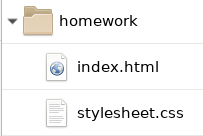
\includegraphics{project}

\section*{Start with \lstinline|index.html|}

This is what an \lstinline|index.html| should contain in the
beginning:

\begin{lstlisting}
<!DOCTYPE html>
<html>
  <head>
    <link rel="stylesheet" type="text/css" href="stylesheet.css">
  </head>
  <body>

  </body>
</html>
\end{lstlisting}

Add your content after the \lstinline|<body>| tag, before
the closing tag \lstinline|</body>|.

\section*{Add a \lstinline|stylesheet.css|}

It can start empty - add the CSS you want. Here is an example:

\begin{lstlisting}
body {
  background-color: lightgrey;
  padding: 2rem;
}
\end{lstlisting}

This will give the whole page a grey background and some spacing. Take
care to use the correct syntax as above - a missing \lstinline|:| or
\lstinline|;| can result in the CSS not working.


\section*{CSS: class selectors }

A class selector in CSS matches all elements with that class. For
example this HTML:

\begin{lstlisting}
<span class="ingredient">Oil</span>
\end{lstlisting}

will be matched by this CSS - note the dot in front of the selector
\lstinline|.ingredient|:

\begin{lstlisting}
.ingredient {
  color: green;
}
\end{lstlisting}

You can freely choose the class name, whatever makes sense to describe
the content it matches. In this example ``ingredient'' is a good choice.

\section*{CSS: element selectors}

An element selector in CSS matches all elements of that kind. For
example this HTML:

\begin{lstlisting}
<p>This is a paragraph.</p>
\end{lstlisting}

will be matched by this CSS, making all \lstinline|p| elements green:

\begin{lstlisting}
p {
  color: green;
}
\end{lstlisting}

\section*{Image}

To include an image on your page, first copy the image file into your
project folder. If it is called \lstinline|myimage.jpg| then add this
HTML:

\begin{lstlisting}
<img src="myimage.jpg">
\end{lstlisting}

Note that there is no closing tag for \lstinline|img|.

\section*{Link}

To make a link to another page, add HTML like this:

\begin{lstlisting}
<a href="someotherpage.html">Some other page</a>
\end{lstlisting}

This will link to a page \lstinline|someotherpage.html| - for this to
work, a file with this name has to exist in the project folder.

\section*{Some CSS properties}

Some useful CSS properties with example values:

\begin{lstlisting}
font-size: 12px;
font-family: Arial, sans-serif;
font-weight: bold;
font-style: italic;
line-height: 1.5em;
background-color: #ef1200;
background: url("myphoto.jpg");
border: 3px solid red;
margin: 3rem;
padding: 20px;
\end{lstlisting}

Experiment with different values to find out what happens. For more
CSS properties, google for ``mdn css properties''.

\vfill

{\small Handout version 2017-06-01}

\end{document}
